\documentclass[10pt,twocolumn]{article}

\usepackage[margin=0.72in]{geometry}
\usepackage{amsmath,amssymb,amsthm,mathtools}
\usepackage{microtype}
\usepackage{times}
\usepackage[hidelinks]{hyperref}
\usepackage{fontawesome5}
\usepackage{enumitem}
\usepackage{graphicx}

\setlist{nosep,leftmargin=*}
\setlength{\columnsep}{0.22in}
\setlength{\parindent}{1em}
\setlength{\parskip}{0pt}

\newtheorem{theorem}{Theorem}
\newtheorem{corollary}{Corollary}
\newtheorem{proposition}{Proposition}
\newtheorem{definition}{Definition}
\newtheorem{remark}{Remark}

\title{\vspace{-1.0em}The Shape of Recursive Redundancy:\\
Velocity Takeoff Kernels for Memoization}
\author{Jonathan R. Landers}
\date{June 2026\\[0.25em]
\href{https://github.com/jonland82/finite-response-kernels}{\faGithub\ Project Repository}}

\begin{document}
\maketitle
\vspace{-1.4em}

\begin{abstract}
Memoization collapses a recursion tree into a directed acyclic graph (DAG) of distinct subproblems.  Standard overlap analysis records the terminal compression rate: if the naive tree has exponential speed \(\alpha\) and the memoized DAG has exponential speed \(\beta\), then the logarithmic overlap velocity tends to \(\alpha-\beta\).  This terminal number is not a complete invariant.  The main result of this paper constructs finite-lag recursive schemas with the same terminal tree speed \(\log 2\), the same polynomial memoized state count, and therefore the same limiting overlap velocity, but with arbitrarily different finite takeoff behavior.  In one schema redundancy becomes visible essentially immediately; in another the approach to the same terminal velocity can have an arbitrarily slow near-periodic transient.  To capture this missing information, the paper introduces the velocity takeoff kernel.  If \(N_n\) is the naive recursion-tree size, \(u_n=\log N_{n+1}-\log N_n\), and \(u_n\to\alpha>0\), then the normalized profile \(F_n=u_n/\alpha\) is a discrete step response \(F_n=(\kappa*H)_n\) of a causal kernel \(\kappa\) of total mass one.  A supporting regularity proposition shows that, for aperiodic finite-lag recurrences, this kernel has exponentially decaying tail and modes determined by the subdominant roots of the recurrence.  The main theorem shows why this kernel is not merely descriptive: it reveals finite redundancy onset that first-order asymptotic overlap invariants cannot measure.
\end{abstract}

\section{Introduction}

Memoization turns repeated recursive calls into shared subproblems.  Before memoization, a recursive computation exposes a tree: equal subproblem labels may appear many times.  After memoization, equal labels are identified and the computation becomes a directed acyclic graph.  Dynamic programming, in Bellman's original formulation \cite{bellman1957}, exploits this quotient.  Michie's memo functions \cite{michie1968} made the same quotient visible as a programming technique.

Let \(N_n\) be the number of calls in the full naive recursion tree on input size \(n\), and let \(M_n\) be the number of distinct subproblems reachable from that input.  The overlap ratio is
\[
        \Theta_n=\frac{N_n}{M_n}.
\]
The logarithmic overlap is \(S_n=\log\Theta_n\), and the overlap velocity is the finite difference
\[
        v_n=S_{n+1}-S_n.
\]
This velocity records the rate at which memoizable redundant work is being created as the input size increases.

The elementary identity
\[
        v_n
        =
        (\log N_{n+1}-\log N_n)
        -
        (\log M_{n+1}-\log M_n)
\]
separates the tree velocity from the DAG velocity.  If \(\log N_n\sim\alpha n\) and \(\log M_n\sim\beta n\), then \(v_n\to\alpha-\beta\).  This is the usual first-order reading: it gives the terminal speed at which overlap is created.

The point of this paper is that the terminal speed is not the whole invariant.  The finite question is different:
\[
        0 \longrightarrow \alpha-\beta.
\]
How does redundancy actually take off?  Does it appear immediately, or only after delayed branches return?  Does the velocity approach its limit monotonically, alternate around it, or ring for a long transient before settling?  These behaviors can occur even when the terminal overlap velocity is the same.

The main separation result makes this precise.  There are finite-lag recursive schemas with the same terminal tree speed \(\alpha=\log2\), the same polynomial memoized state count \(M_n=O(n)\), and hence the same limiting overlap velocity \(\log2\), but with different takeoff classes.  The immediate binary recurrence reaches its terminal velocity at once up to boundary effects.  A second aperiodic family has the same terminal velocity and the same one-dimensional memoized state set, while its modal radius can be made larger than \(1-\delta\) for any \(\delta>0\).  Thus the finite onset of redundancy is not determined by \(\alpha\), by \(\beta\), or by the growth class of the memoized DAG.

To measure the missing information, define the tree velocity
\[
        u_n=\log N_{n+1}-\log N_n.
\]
When \(u_n\to\alpha>0\), the normalized curve \(F_n=u_n/\alpha\) is the velocity takeoff profile.  Its finite difference
\[
        \kappa_n=F_n-F_{n-1},\qquad F_{-1}=0,
\]
is the causal takeoff kernel.  Equivalently, \(F_n=(\kappa*H)_n\), where \(H\) is the discrete step function.  The definition is simple; the content is that finite-lag recurrences give kernels whose tails and oscillations are controlled by the subdominant roots of the recurrence.

There are therefore two steps in the argument.  First, a regularity proposition translates standard finite-lag recurrence asymptotics into the language of takeoff kernels: the kernel has total mass one, exponential settling, and recurrence-root modes.  Second, the main theorem shows that this extra finite-response information is necessary: the kernel distinguishes recursive schemas that first-order overlap invariants cannot distinguish.

The contribution is not a new solution method for linear recurrences.  Classical recurrence theory, generating functions, and branching processes already contain the dominant-root equation \cite{bellman1952,biggins1977,flajolet2009}.  The contribution is the overlap-velocity interpretation and the separation it enables.  Recursive inefficiency has a response shape.  Memoization removes accumulated overlap, but the way that overlap becomes visible is itself structured.

This viewpoint sits before the fine-grained complexity question of how fast the collapsed dynamic program can be evaluated \cite{backurs2015,abboud2015,bringmann2015,kunnemann2017,alman2024,jin2024}.  The takeoff kernel describes the redundant recursive response that creates the DAG in the first place.

\section{Overlap Velocity}

All logarithms are natural logarithms.  The input size is a nonnegative integer \(n\).  For a recursive computation on size \(n\), let \(N_n\) be the number of calls in the naive recursion tree, counting repeated subproblems with multiplicity.  Let \(U_n\) be the set of distinct subproblem labels reached from that input, and let
\[
        M_n=|U_n|
\]
be the number of distinct subproblems.  The overlap ratio \(\Theta_n=N_n/M_n\) is the average number of tree appearances per distinct subproblem.

Define the logarithmic overlap \(S_n=\log \Theta_n\).  The overlap velocity is
\[
        v_n=S_{n+1}-S_n.
\]
It is useful to name the two components of this velocity.  The tree velocity is
\[
        u_n=\log N_{n+1}-\log N_n,
\]
and the DAG velocity is
\[
        w_n=\log M_{n+1}-\log M_n.
\]
Then
\[
        v_n=u_n-w_n.
\]
Thus memoization removes not only accumulated work but also a velocity profile.  If \(M_n\) is polynomial in \(n\), then \(w_n\to 0\), and the overlap takeoff is essentially the tree takeoff.  If \(M_n\) is exponential, then the DAG itself has a competing velocity.

\section{Finite-Lag Recursion}

A finite-lag recursive schema is defined by a finite nonempty set \(J\subseteq\{1,2,3,\ldots\}\) and a positive integer \(a_j\) for each \(j\in J\).  The integer \(j\) is a size decrement, and \(a_j\) is the number of recursive calls from size \(n\) to size \(n-j\).  The naive tree size is modeled by
\begin{equation}\label{eq:tree}
        N_n
        =
        1+\sum_{j\in J}a_jN_{n-j},
        \qquad n\ge 1,
\end{equation}
with boundary convention \(N_m=1\) for \(m\le 0\).  The boundary changes constants but not the takeoff modes.

The total branching number is
\[
        A=\sum_{j\in J}a_j.
\]
When \(A=1\), the recursion is path-like and has no positive exponential tree velocity.  The interesting redundant case is \(A>1\).  Define the polynomial
\[
        Q(z)=1-\sum_{j\in J}a_jz^j.
\]
There is a unique positive number \(\rho\in(0,1)\) satisfying
\begin{equation}\label{eq:rho}
        Q(\rho)=0,
        \quad\text{equivalently}\quad
        \sum_{j\in J}a_j\rho^j=1.
\end{equation}
The terminal tree speed is
\[
        \alpha=-\log \rho.
\]

The normalized call-decrement distribution is the recursion kernel \(K\) defined by
\[
        K_j=\frac{a_j}{A},
        \qquad j\in J.
\]
This kernel records where the raw recursive branches land.  The takeoff kernel introduced below is different: it records how the observed velocity approaches its terminal value.

\section{Regularity of the Takeoff Kernel}

Let \(H_n\) denote the discrete step function, defined by \(H_n=1\) for \(n\ge 0\) and \(H_n=0\) for \(n<0\).  If a sequence \(\kappa=(\kappa_n)_{n\in\mathbb{Z}}\) satisfies \(\kappa_n=0\) for \(n<0\), its step response is
\[
        (\kappa * H)_n=\sum_{t=0}^{n}\kappa_t.
\]
The sequence is causal because only present and past indices contribute.

\begin{definition}[Velocity takeoff kernel]
Assume the tree velocity \(u_n=\log N_{n+1}-\log N_n\) converges to a positive limit \(\alpha\).  The normalized takeoff profile is
\[
        F_n=\frac{u_n}{\alpha},
        \qquad n\ge 0.
\]
Set \(F_{-1}=0\).  The velocity takeoff kernel is the causal sequence \(\kappa\) defined by
\[
        \kappa_n=F_n-F_{n-1}\quad(n\ge 0),
        \qquad
        \kappa_n=0\quad(n<0).
\]
\end{definition}

By definition, \(F_n=(\kappa*H)_n\).  The following proposition is the technical normalization step.  It records that finite-lag recursion gives a well-behaved finite-response kernel: the profile settles to mass one at a rate controlled by the recurrence roots.  This is mostly classical recurrence theory, but it makes the later separation statement precise.

\begin{proposition}[Finite-lag takeoff regularity]\label{prop:takeoff}
Consider the finite-lag schema \eqref{eq:tree} with total branching number \(A>1\).  Let \(Q(z)=1-\sum_{j\in J}a_jz^j\), let \(\rho\in(0,1)\) be the positive root in \eqref{eq:rho}, and let \(\alpha=-\log\rho\).  Assume the greatest common divisor of the integers in \(J\) is \(1\).  Then the tree velocity \(u_n=\log N_{n+1}-\log N_n\) satisfies
\[
        \lim_{n\to\infty}u_n=\alpha.
\]
The takeoff kernel \(\kappa\) has total mass one:
\[
        \sum_{n=0}^{\infty}\kappa_n=1.
\]
Moreover, there are constants \(C>0\) and \(\lambda\in(0,1)\) such that
\[
        |F_n-1|\le C\lambda^n
        \quad\text{and}\quad
        |\kappa_n|\le C\lambda^n
\]
for all sufficiently large \(n\).  If \(\zeta\) is a non-dominant root of \(Q\), then its contribution to the leading correction has mode \((\rho/\zeta)^n\) whenever that root is among the closest singularities to \(\rho\).  Thus negative or complex non-dominant roots produce alternating or oscillatory takeoff, while positive real non-dominant roots produce monotone exponential smoothing when their coefficients have the appropriate sign.
\end{proposition}

\begin{proof}
The ordinary generating function \(G(z)=\sum_{n\ge0}N_nz^n\) is rational.  The recurrence \eqref{eq:tree} gives a denominator of the form \((1-z)Q(z)\), up to numerator factors determined by the boundary convention.  Since \(A>1\), the positive root \(\rho\) of \(Q\) lies inside the unit disk.  Since the coefficients \(a_j\) are nonnegative and \(\gcd(J)=1\), the root \(\rho\) is the unique singularity of smallest modulus.  This is the standard aperiodic case for nonnegative linear recurrences; see the transfer theorems in analytic combinatorics \cite{flajolet2009}.

Therefore
\[
        N_n=C_0\rho^{-n}(1+\varepsilon_n)
\]
for some constant \(C_0>0\), where \(\varepsilon_n\to0\) exponentially.  More precisely, the exponential rates in \(\varepsilon_n\) are ratios \((\rho/\zeta)^n\), where \(\zeta\) ranges over singularities of \(G\) other than \(\rho\), including non-dominant roots of \(Q\) and the singularity at \(z=1\).  Hence
\[
        u_n
        =
        \log\frac{N_{n+1}}{N_n}
        =
        -\log\rho
        +
        \log\frac{1+\varepsilon_{n+1}}{1+\varepsilon_n}.
\]
The second term tends to zero exponentially, so \(u_n\to\alpha\).  Dividing by \(\alpha\) gives \(F_n\to1\), and the definition \(\kappa_n=F_n-F_{n-1}\) gives
\[
        \sum_{n=0}^{m}\kappa_n=F_m.
\]
Letting \(m\to\infty\) proves \(\sum_{n\ge0}\kappa_n=1\).  Since both \(F_n-1\) and \(F_{n-1}-1\) decay exponentially, so does \(\kappa_n\).  The modal statement follows from the partial-fraction expansion of the rational generating function.
\end{proof}

\begin{remark}
Proposition~\ref{prop:takeoff} does not say that \(\kappa_n\) is always nonnegative.  If \(\kappa_n\ge0\) for all \(n\), the takeoff is a passive smoothing kernel in the strict sense: the normalized velocity rises as a cumulative distribution.  If some \(\kappa_n\) are negative, the response is signed.  That is still informative.  Negative mass marks overshoot, alternating corrections, or ringing caused by competing recursive scales.
\end{remark}

\begin{corollary}[Settling time and signed response]\label{cor:settling}
Under the hypotheses of Proposition~\ref{prop:takeoff}, fix a tolerance \(\varepsilon>0\).  Define the \(\varepsilon\)-settling time \(T_\varepsilon\) to be the smallest integer \(T\) such that
\[
        |F_n-1|\le\varepsilon
        \quad\text{for every } n\ge T.
\]
Then \(T_\varepsilon=O(\log(1/\varepsilon))\) as \(\varepsilon\downarrow0\).  If the takeoff kernel \(\kappa\) is nonnegative, then \(F_n\) is monotone nondecreasing and \(F_n\) is the cumulative distribution function of a probability law on \(\mathbb{N}_0\).  If \(\kappa\) has negative entries, the excess signed response
\[
        R(\kappa)=\sum_{n\ge0}|\kappa_n|-1
\]
is finite and measures the amount of overshoot or ringing in the normalized velocity response.  The value of \(R(\kappa)\) depends on the finite prefix of \(\kappa\), and therefore on the chosen base-case convention, but its tail is controlled by the recurrence modes.
\end{corollary}

\begin{proof}
The exponential estimate \(|F_n-1|\le C\lambda^n\) from Proposition~\ref{prop:takeoff} implies that \(|F_n-1|\le\varepsilon\) once \(n\ge \log(C/\varepsilon)/\log(1/\lambda)\), proving the settling-time bound.  If every \(\kappa_n\) is nonnegative, then \(F_n=\sum_{t=0}^n\kappa_t\) is nondecreasing, and Proposition~\ref{prop:takeoff} gives \(\sum_{n\ge0}\kappa_n=1\), so \(\kappa\) is a probability law.  If signs occur, the exponential bound on \(\kappa_n\) implies \(\sum_n|\kappa_n|<\infty\), so \(R(\kappa)\) is finite.
\end{proof}

Corollary~\ref{cor:settling} gives two quantities that can be measured without solving the recurrence exactly.  The settling time says how long the recursion behaves like a startup transient before its asymptotic overlap velocity is visible.  The signed response \(R(\kappa)\) distinguishes a passive rise from a response that overshoots and returns.  These are not traditional big-\(O\) costs; they are shape parameters for redundant computation.

The settling time also gives a practical decision rule for bounded inputs.  Fix a tolerance \(\varepsilon\).  If the input range of interest lies mostly below \(T_\varepsilon\), then the recursion is still in its startup response: asymptotic overlap exists, but it is not yet the behavior seen by the computation.  If the range extends well beyond \(T_\varepsilon\), and the DAG velocity \(w_n\) is small relative to the tree velocity, then memoization is exposing persistent redundancy rather than only boundary effects.  This is not a machine-independent runtime theorem, but it is an intrinsic threshold for when stable overlap has begun.

\section{Main Separation}

Proposition~\ref{prop:takeoff} makes the kernel legitimate.  This section gives the reason to care about it: terminal overlap data do not determine finite redundancy onset.  The missing information is carried by the modal structure of the takeoff profile, and the main theorem shows that this information cannot be recovered from the usual first-order invariants.

Let \(G(z)=\sum_{n\ge0}N_nz^n\) be the generating function of the tree sizes, and let \(\rho=e^{-\alpha}\) be its dominant positive singularity.  Let \(\mathcal{Z}\) be the set of singularities of \(G\) other than \(\rho\).  In the finite-lag model, these singularities are among the roots of \(Q(z)\) together with \(z=1\), after removing any cancellations caused by the numerator.  Define the modal radius
\[
        \lambda_\star
        =
        \max_{\zeta\in\mathcal{Z}}
        \left|\frac{\rho}{\zeta}\right|.
\]
The aperiodic assumption in Proposition~\ref{prop:takeoff} implies \(\lambda_\star<1\).  A modal radius near zero means fast settling.  A modal radius near one means a long finite transient before the terminal velocity is visible.

\begin{corollary}[Modal radius]\label{cor:modal}
For every number \(\lambda\) satisfying \(\lambda_\star<\lambda<1\), the normalized takeoff profile obeys
\[
        |F_n-1|=O(\lambda^n).
\]
If a singularity \(\zeta\in\mathcal{Z}\) with \(|\rho/\zeta|=\lambda_\star\) has nonzero coefficient in the partial-fraction expansion of \(G\), then the takeoff profile has a leading correction of order \(\lambda_\star^n\), possibly multiplied by a polynomial in \(n\) if the singularity is multiple.
\end{corollary}

\begin{proof}
This is the modal part of Proposition~\ref{prop:takeoff} stated as an invariant.  The rational generating function has a partial-fraction expansion.  Dividing the contribution of a non-dominant singularity \(\zeta\) by the dominant term \(\rho^{-n}\) produces the ratio \((\rho/\zeta)^n\).  The largest such modulus controls the slowest exponential settling mode, unless its coefficient vanishes.
\end{proof}

Thus two recursive schemas can have the same terminal exponent \(\alpha\) but different finite-response behavior.  One may reach its terminal velocity in a few input steps; another may have a long startup tail.  One may approach monotonically; another may alternate around the limit.  Big-\(O\) notation usually discards those differences as lower-order terms.  The kernel view keeps them because they are algorithmically visible in finite input ranges and experimentally visible in traces of recursive programs.

This is also where the analogy with finite physical response is closest.  The number \(\alpha\) is the final velocity.  The modal radius \(\lambda_\star\), the settling time \(T_\varepsilon\), and the signed response \(R(\kappa)\) describe the route to that velocity.  For recursive algorithms, that route records when repeated subproblems begin to dominate.  A recurrence whose redundancy takes off only after a long delay may behave like an iterative computation on small inputs even if its terminal exponent is positive.

The next theorem is the main contribution.  It says that the takeoff kernel is not a cosmetic repackaging of the terminal exponent: two recurrences can agree on the terminal tree speed, on the memoized state-growth class, and on the limiting overlap velocity, while disagreeing arbitrarily strongly on finite takeoff.

\begin{theorem}[Main separation: first-order overlap invariants do not determine takeoff]\label{thm:separation}
There are finite-lag recursive schemas with the same terminal tree speed \(\alpha=\log2\), the same polynomial memoized state count \(M_n=O(n)\), and therefore the same limiting overlap velocity \(\log2\), but with different takeoff classes.  In particular, the immediate binary schema
\[
        N_n=1+2N_{n-1}
\]
has modal radius \(1/2\).  For every \(\delta>0\), there is an aperiodic schema with the same terminal speed and polynomial memoized state count whose modal radius is greater than \(1-\delta\).
\end{theorem}

\begin{proof}
The immediate binary schema has \(Q(z)=1-2z\), dominant root \(\rho=1/2\), and no non-dominant root of \(Q\).  The affine recurrence contributes the singularity \(z=1\), so the modal radius is \(\rho/1=1/2\).  Its reachable one-dimensional subproblem labels are among \(0,1,\ldots,n\), so \(M_n=O(n)\).

For the slow family, fix an integer \(L\ge2\) and define
\[
        N_n=1+(2^{L}-1)N_{n-L}+2N_{n-L-1}.
\]
Here \(J=\{L,L+1\}\), so the schema is aperiodic.  Its characteristic polynomial is
\[
        Q_L(z)=1-(2^{L}-1)z^L-2z^{L+1}.
\]
Since
\[
        (2^{L}-1)2^{-L}+2\cdot2^{-(L+1)}=1,
\]
the positive dominant root is again \(\rho=1/2\), and the terminal tree speed is \(\log2\).  The reachable labels are still one-dimensional, so \(M_n\le n+1\) and the memoized DAG exponent is \(0\).

It remains to see that the modal radius can approach one.  Compare \(Q_L\) with the periodic polynomial
\[
        P_L(z)=1-2^{L}z^L.
\]
The non-real roots of \(P_L\) are \((1/2)e^{2\pi i k/L}\), \(1\le k<L\), all on the circle of radius \(1/2\).  Moreover
\[
        Q_L(z)-P_L(z)=z^L(1-2z),
\]
which is exponentially small near those roots.  By the standard continuity of simple polynomial roots, equivalently by Rouch\'e's theorem on small circles around the roots of \(P_L\), \(Q_L\) has a non-dominant root \(\zeta_L\) with
\[
        \left|\zeta_L-\frac12e^{2\pi i/L}\right|\to0
        \quad\text{as }L\to\infty.
\]
With the boundary convention \(N_m=1\) for \(m\le0\), the numerator of \(G_L(z)\) is relatively prime to \(Q_L(z)\); equivalently, these nearby roots are genuine non-dominant singularities of the tree-size generating function.  The aperiodic nonnegative recurrence has no other root on the dominant circle, so \(|\zeta_L|>1/2\), but the displayed convergence gives \(|\zeta_L|\to1/2\).  Hence
\[
        \frac{\rho}{|\zeta_L|}\to1.
\]
Choosing \(L\) large enough makes the modal radius greater than \(1-\delta\).
\end{proof}

Theorem~\ref{thm:separation} is the main separation.  The two families agree on the usual exponential tree rate, on the growth class of the memoized state graph, and on limiting overlap velocity.  They differ in when the asymptotic redundancy regime becomes visible.  No statement using only \(\alpha\), \(\beta\), or the growth class of \(M_n\) can see that difference.  The takeoff kernel can.  Figure~\ref{fig:separation} shows the separation numerically: the terminal overlap velocity is the same, but the finite response can settle immediately or ring for a long transient.

\begin{figure*}[t]
  \centering
  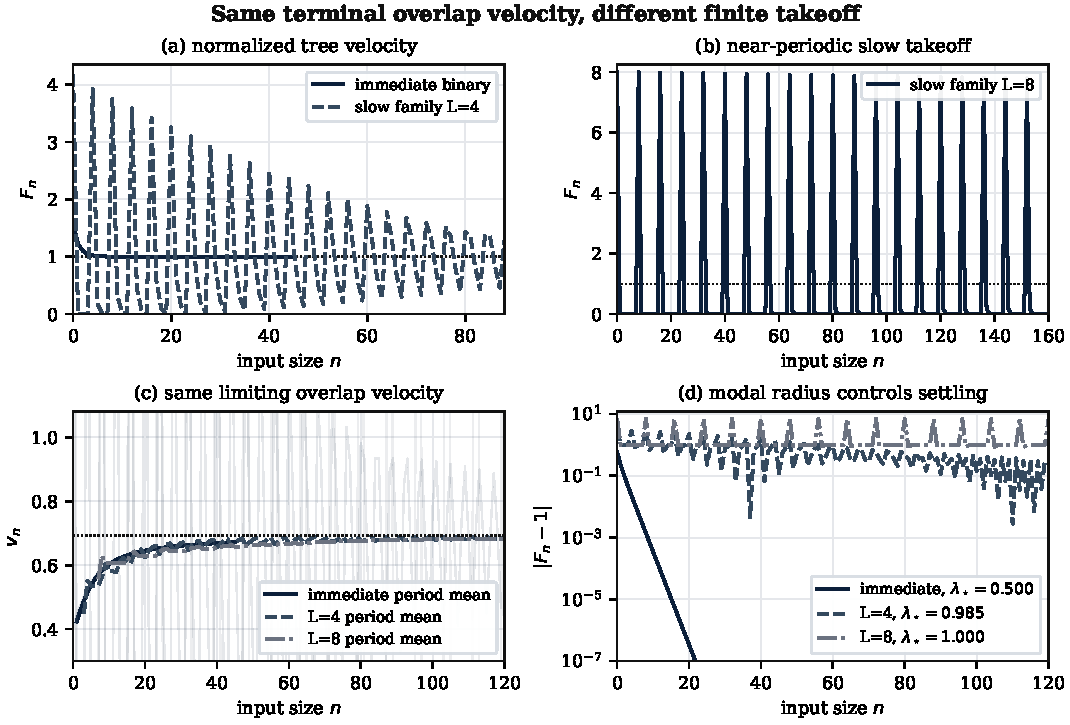
\includegraphics[width=0.94\textwidth]{velocity_takeoff_figures/fig1_separation.pdf}
  \caption{Numerical view of Theorem~\ref{thm:separation}.  The immediate binary recurrence and the delayed families have the same terminal tree speed \(\log2\), the same polynomial memoized state growth, and the same limiting overlap velocity, but their takeoff profiles and modal radii are visibly different.}
  \label{fig:separation}
\end{figure*}

The same modal language also gives a quantitative tail estimate for signed response.  This bound is not the main separation, but it is useful when comparing measured kernels after discarding a finite warmup prefix.

\begin{corollary}[Tail signed-response bound]\label{cor:tail}
Suppose the correction to the normalized takeoff profile has the form
\[
        F_n-1=\sum_{r=1}^{m}c_r\theta_r^n+O(\eta^n),
        \qquad 0\le\eta<\max_r|\theta_r|<1,
\]
where the complex modes are listed with their conjugates so that \(F_n\) is real.  For the tail response
\[
        R_N(\kappa)=\sum_{n\ge N}|\kappa_n|,
\]
one has
\[
        R_N(\kappa)
        \le
        \sum_{r=1}^{m}
        \frac{|c_r|\,|1-\theta_r|\,|\theta_r|^{N-1}}{1-|\theta_r|}
        +O(\eta^N).
\]
\end{corollary}

\begin{proof}
Since \(\kappa_n=F_n-F_{n-1}\), the mode \(c_r\theta_r^n\) contributes \(c_r(\theta_r-1)\theta_r^{n-1}\).  Summing absolute values over \(n\ge N\) gives a geometric bound for each mode.  The lower modes contribute \(O(\eta^N)\).
\end{proof}

\section{Terminal Speed as Entropy}

Proposition~\ref{prop:takeoff} describes the route to the terminal speed.  The terminal speed itself has a compact entropy form, using the standard entropy and relative-entropy notation of information theory \cite{cover2006}.  Let \(p=(p_j)_{j\in J}\) be a probability distribution on the decrement set \(J\).  Its entropy is
\[
        H(p)=-\sum_{j\in J}p_j\log p_j,
\]
and its relative entropy from the recursion kernel \(K\) is
\[
        D(p\|K)=\sum_{j\in J}p_j\log\frac{p_j}{K_j}.
\]
The mean decrement under \(p\) is
\[
        \mu(p)=\sum_{j\in J}jp_j.
\]

\begin{corollary}[Entropy formula for terminal speed]\label{cor:entropy}
For the finite-lag schema above, the terminal speed \(\alpha=-\log\rho\) satisfies
\[
        \alpha
        =
        \max_{p}
        \frac{\log A-D(p\|K)}{\mu(p)},
\]
where the maximum is over all probability distributions \(p\) on \(J\).  The maximizing distribution is
\[
        p_j^\star=a_je^{-\alpha j},
        \qquad j\in J.
\]
\end{corollary}

\begin{proof}
Equation \eqref{eq:rho} says that \(q_j=a_je^{-\alpha j}\) sums to one, so \(q=(q_j)_{j\in J}\) is a probability distribution.  For any \(p\), nonnegativity of \(D(p\|q)\) gives
\[
        0
        \le
        \sum_{j\in J}p_j\log\frac{p_j}{a_je^{-\alpha j}}
        =
        -H(p)-\sum_{j\in J}p_j\log a_j+\alpha\mu(p).
\]
Thus
\[
        \alpha
        \ge
        \frac{H(p)+\sum_{j\in J}p_j\log a_j}{\mu(p)}.
\]
Equality holds when \(p=q\).  Since \(a_j=AK_j\), the numerator equals \(\log A-D(p\|K)\), which proves the displayed formula.
\end{proof}

The corollary says that the terminal speed is branching entropy per unit size after paying a mismatch penalty.  Proposition~\ref{prop:takeoff} adds the missing finite-response statement: the recurrence roots determine how that terminal speed is approached.

\section{Takeoff Types}

\paragraph{No takeoff: linear recursion.}
For one call from \(n\) to \(n-1\), the set of decrements is \(J=\{1\}\), the multiplicity is \(a_1=1\), and \(A=1\).  The tree is a path, so \(N_n\) grows linearly rather than exponentially.  There is stack depth, but no positive overlap velocity.

\paragraph{Immediate takeoff: binary one-step recursion.}
For two calls from \(n\) to \(n-1\), \(J=\{1\}\) and \(a_1=2\).  The root equation is \(2e^{-\alpha}=1\), so \(\alpha=\log2\).  Apart from boundary effects, the velocity is already at the binary speed.  The takeoff kernel is concentrated near the origin.

\paragraph{Delayed takeoff: binary lag \(L\).}
For two calls from \(n\) to \(n-L\), \(J=\{L\}\) and \(a_L=2\).  The terminal speed per unit of the original input coordinate is
\[
        \alpha=\frac{\log2}{L}.
\]
The greatest common divisor condition fails when \(L>1\), so the raw sequence has residue-class effects.  In the coarse coordinate \(m=n/L\), the recurrence is immediate binary branching.  In the original coordinate, the response has dead time: recursive mass cannot return until the lag has been paid.

\paragraph{Monotone envelope: Fibonacci.}
Naive Fibonacci has one call to \(n-1\) and one call to \(n-2\).  Thus \(J=\{1,2\}\) and \(a_1=a_2=1\).  The terminal speed solves
\[
        e^{-\alpha}+e^{-2\alpha}=1,
\]
so \(\alpha=\log\varphi\), where \(\varphi=(1+\sqrt5)/2\).  Because \(N_n\) counts all call nodes, the affine \(+1\) in the recurrence contributes the singularity \(z=1\).  This gives a monotone correction of order \(\rho^n=\varphi^{-n}\), where \(\rho=1/\varphi\).  The polynomial \(Q(z)=1-z-z^2\) also has the non-dominant root \(\zeta=-\varphi\), giving the alternating mode
\[
        \left(\frac{\rho}{\zeta}\right)^n
        =
        \left(-\varphi^{-2}\right)^n.
\]
Thus Fibonacci is not a leading-ringing example under node counting.  Its leading finite-response behavior is monotone settling, with a faster alternating ripple underneath.  If one counts only leaves, the \(z=1\) contribution disappears and the alternating mode becomes leading.  Figure~\ref{fig:fibonacci-kernel} illustrates this boundary-convention effect: the tail modes are the same recurrence information, but the visible kernel prefix changes.

\begin{figure*}[t]
  \centering
  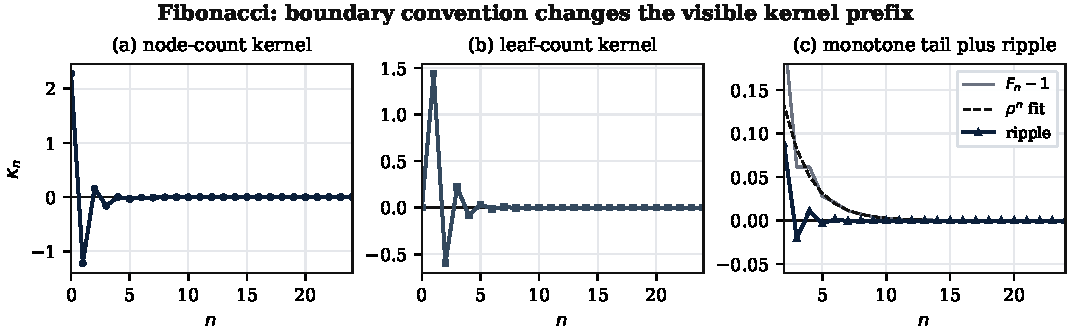
\includegraphics[width=0.90\textwidth]{velocity_takeoff_figures/fig2_fibonacci.pdf}
  \caption{Fibonacci takeoff depends on the counting convention.  Under node counting, the affine term contributes a monotone \(z=1\) correction; under leaf counting, that contribution disappears and the alternating mode is more visible.}
  \label{fig:fibonacci-kernel}
\end{figure*}

\paragraph{Leading ringing: near-periodic delayed branching.}
The slow family in Theorem~\ref{thm:separation} has roots \(\zeta_L\) near \((1/2)e^{2\pi i/L}\), while the dominant root is \(\rho=1/2\).  Its leading mode is approximately
\[
        \left(\frac{\rho}{\zeta_L}\right)^n
        \approx
        e^{-2\pi i n/L}
\]
with modulus just below one.  This is genuine leading ringing: the complex mode dominates the \(z=1\) monotone correction, whose modulus is only \(1/2\), and the oscillation can be made arbitrarily slow by increasing \(L\).

\paragraph{Mixed takeoff: parallel channels.}
Suppose one channel branches quickly and another channel returns after a longer lag.  If the fast channel has multiplicities \(b_j\) and the slow channel has multiplicities \(c_j\), the combined multiplicity is \(a_j=b_j+c_j\).  The recursion kernel \(K_j=a_j/A\) is a mixture weighted by branch counts.  The takeoff kernel need not be the same mixture, because the recurrence roots interact globally.  This is where multi-stage response shapes appear: a fast initial rise followed by a slower settling tail.

\paragraph{Diffusive takeoff: grid dynamic programs.}
Some dynamic programs are not one-dimensional finite-lag recurrences.  For lattice paths, the number of paths to \((i,j)\) satisfies \(P_{i,j}=P_{i-1,j}+P_{i,j-1}\).  Along the diagonal, \(P_{n,n}=\binom{2n}{n}\), so
\[
        \log P_{n,n}=2n\log2-\frac12\log n+O(1).
\]
The velocity approaches \(2\log2\) with an algebraic correction of order \(1/n\), not an exponential correction.  This is a different smoothing class.  It is closer to a diffusive kernel than to a finite-dimensional linear recurrence kernel, and it suggests why multidimensional DP grids deserve a separate theorem.  Figure~\ref{fig:decay-class} contrasts this algebraic settling with the exponential settling from finite-lag recurrences.

\begin{figure}[t]
  \centering
  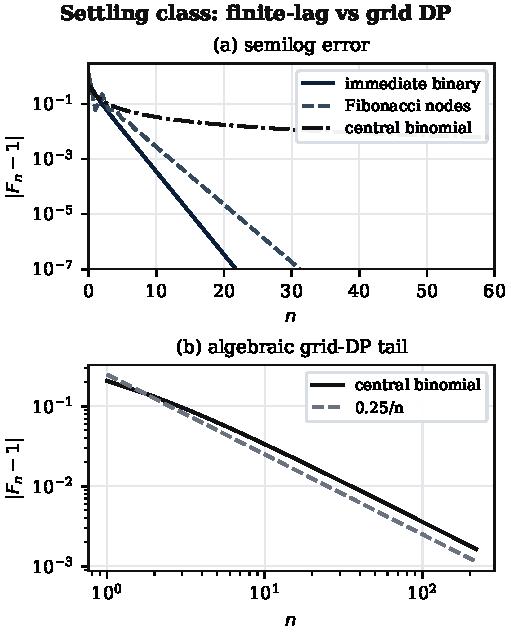
\includegraphics[width=0.86\columnwidth]{velocity_takeoff_figures/fig3_decay_class.pdf}
  \caption{Finite-lag recurrences settle exponentially, while diagonal grid-DP path counts have an algebraic \(1/n\)-scale tail.}
  \label{fig:decay-class}
\end{figure}

\section{Overlap Corollary}

The regularity proposition describes \(u_n\), the tree velocity.  The overlap velocity is \(v_n=u_n-w_n\), where \(w_n=\log M_{n+1}-\log M_n\) is the DAG velocity.

\begin{corollary}[Overlap takeoff]\label{cor:overlap}
Assume \(u_n\to\alpha\) and \(w_n\to\beta\), where \(\alpha\) and \(\beta\) are nonnegative real numbers.  Then the overlap velocity satisfies
\[
        v_n\to\alpha-\beta.
\]
If \(\alpha>0\), \(F_n=u_n/\alpha\) is the tree takeoff profile.  If \(\beta>0\), \(G_n=w_n/\beta\) is the DAG takeoff profile.  Then
\[
        v_n=\alpha F_n-\beta G_n.
\]
In particular, when \(M_n\) is polynomial, \(\beta=0\), and the overlap takeoff inherits the tree takeoff.
\end{corollary}

\begin{proof}
The identity \(v_n=u_n-w_n\) gives the limit.  The displayed decomposition follows by substituting \(u_n=\alpha F_n\) and \(w_n=\beta G_n\) when the normalizations are defined.
\end{proof}

The error from terminal overlap velocity is
\[
        v_n-(\alpha-\beta)
        =
        \alpha(F_n-1)-\beta(G_n-1).
\]
Thus, when both sides have modal expansions, the overlap takeoff is controlled by the slower of the tree and DAG modes, unless the leading coefficients cancel.  For Fibonacci, \(M_n=n+1\), so \(w_n=\log(n+2)-\log(n+1)\to0\).  The overlap velocity therefore inherits the tree profile: monotone settling with a smaller alternating ripple, converging to \(\log\varphi\).  For a DP whose state graph is itself exponential, the observed overlap takeoff is genuinely a difference between two response curves.

\section{Relation to Algorithms}

The takeoff kernel belongs to the first step in a standard algorithmic pipeline:
\[
\begin{aligned}
        \text{naive recursion}
        &\xrightarrow{\text{memoization}}
        \text{subproblem DAG},\\
        \text{subproblem DAG}
        &\xrightarrow{\text{structure}}
        \text{optimized evaluation}.
\end{aligned}
\]
The kernel measures how redundant work appears before the quotient by equal labels.  It is a diagnostic for finite-input memoization behavior, not a lower bound on the best algorithm for evaluating the resulting DAG.

This distinction is important in fine-grained complexity.  Conditional lower bounds for edit distance, LCS, dynamic time warping, and related dynamic programs show that strongly subquadratic exact algorithms would contradict SETH, the Strong Exponential Time Hypothesis \cite{impagliazzo2001,backurs2015,abboud2015,bringmann2015}.  Recent bounded weighted edit-distance results sharpen the same distinction in dynamic settings \cite{boneh2025}.  Those results concern the collapsed dynamic program, not simply the waste in a top-down recursion without memoization.

Recent positive results also live mostly after the collapse.  K\"unnemann, Paturi, and Schneider \cite{kunnemann2017} identify structure in one-dimensional dynamic programs.  Alman, Turok, Yu, and Zhang \cite{alman2024} use tensor rank and slice rank to analyze speedups for broad classes of dynamic programs.  Jin's near-quadratic algorithm for 0-1 knapsack \cite{jin2024}, and recent work on higher-dimensional knapsack and convolution \cite{grage2025}, change the frontier for classical DP evaluation.  The takeoff-kernel view is complementary: it asks what kind of redundant recursive response created the DAG in the first place.

\section{Experimental Agenda}

The separation theorem suggests a direct measurement program.  For a recursive implementation, record \(N_n\), the number of naive calls, and \(M_n\), the number of distinct labels reached under memoization.  Then compute
\begin{align*}
        u_n&=\log N_{n+1}-\log N_n,\\
        w_n&=\log M_{n+1}-\log M_n,\\
        v_n&=u_n-w_n .
\end{align*}
When \(u_n\) has an apparent terminal value \(\alpha\), form \(F_n=u_n/\alpha\) and \(\kappa_n=F_n-F_{n-1}\).  The plotted kernel should reveal whether the recurrence has immediate, delayed, oscillatory, mixed, or diffusive takeoff.  The first few entries of \(\kappa\) depend on base cases and boundary conventions, so experiments should report that convention.  For near-periodic schemas or cases with \(\lambda_\star\) close to one, discarding a warmup prefix may not reveal a settled tail within the observable window; experiments should also report the response envelope or a period-averaged velocity.

The first benchmark family should be deliberately simple: Fibonacci, \(k\)-bonacci, delayed binary recursion, lattice paths, edit distance, context-free parsing recurrences, and memoized search problems with changing branching factors.  For CYK-style parsing and related dynamic programs, even I/O behavior is a separate post-collapse question \cite{destefani2025}.  The value of the experiment is not to rediscover their asymptotic costs.  It is to show that recursive redundancy has a measurable response shape, and that this shape is stable enough to classify algorithms before fine-grained optimization begins.

\section{Conclusion}

The limiting overlap velocity \(\alpha-\beta\) is only the terminal reading of a richer finite-response object.  In a finite-lag recursive schema, the tree velocity \(u_n=\log N_{n+1}-\log N_n\) approaches its terminal value \(\alpha\) through a causal takeoff profile \(F_n\).  The kernel \(\kappa_n=F_n-F_{n-1}\) has total mass one and, in the aperiodic finite-lag case, exponentially decaying tail controlled by the subdominant recurrence roots.

The main point is Theorem~\ref{thm:separation}: first-order overlap invariants do not determine takeoff.  Two recursive schemas can have the same exponential tree growth, the same polynomial memoized state count, and the same limiting overlap velocity, while one displays immediate redundancy takeoff and another has an arbitrarily slow near-periodic transient.  The kernel is therefore not just a repackaging of the terminal exponent.  It is a second-order invariant that records when memoizable redundancy becomes visible.

This gives a sharper vocabulary for recursive inefficiency.  A recurrence can have immediate takeoff, delayed takeoff, damped ringing, mixed-stage smoothing, or diffusive smoothing in a higher-dimensional state space.  Memoization removes accumulated overlap, but the way overlap appears is itself structured.  Recursion is not inefficient merely because it is recursion; it becomes inefficient when its takeoff kernel drives tree velocity faster than the distinct-subproblem DAG can grow.

\footnotesize
\begin{thebibliography}{99}

\bibitem{abboud2015}
A.~Abboud, A.~Backurs, and V.~Vassilevska Williams.
\newblock Tight hardness results for LCS and other sequence similarity measures.
\newblock In \emph{Proceedings of FOCS 2015}, pages 59--78, 2015.

\bibitem{alman2024}
J.~Alman, E.~Turok, H.~Yu, and H.~Zhang.
\newblock Tensor ranks and the fine-grained complexity of dynamic programming.
\newblock In \emph{Proceedings of ITCS 2024}, LIPIcs 287, article 4, 2024.

\bibitem{backurs2015}
A.~Backurs and P.~Indyk.
\newblock Edit distance cannot be computed in strongly subquadratic time (unless SETH is false).
\newblock In \emph{Proceedings of STOC 2015}, pages 51--58, 2015.

\bibitem{bellman1952}
R.~Bellman and T.~E. Harris.
\newblock On age-dependent binary branching processes.
\newblock \emph{Annals of Mathematics}, 55(2):280--295, 1952.

\bibitem{bellman1957}
R.~Bellman.
\newblock \emph{Dynamic Programming}.
\newblock Princeton University Press, 1957.

\bibitem{biggins1977}
J.~D. Biggins.
\newblock Martingale convergence in the branching random walk.
\newblock \emph{Journal of Applied Probability}, 14(1):25--37, 1977.

\bibitem{boneh2025}
I.~Boneh, E.~Gorbachev, and T.~Kociumaka.
\newblock Bounded weighted edit distance: Dynamic algorithms and matching lower bounds.
\newblock In \emph{Proceedings of ESA 2025}, LIPIcs 351, article 45, 2025.

\bibitem{bringmann2015}
K.~Bringmann and M.~K\"unnemann.
\newblock Quadratic conditional lower bounds for string problems and dynamic time warping.
\newblock In \emph{Proceedings of FOCS 2015}, pages 79--97, 2015.

\bibitem{cover2006}
T.~M. Cover and J.~A. Thomas.
\newblock \emph{Elements of Information Theory}.
\newblock Wiley, second edition, 2006.

\bibitem{destefani2025}
L.~De~Stefani and V.~Gupta.
\newblock On the I/O complexity of the Cocke-Younger-Kasami algorithm and of a family of related dynamic programming algorithms.
\newblock In \emph{Proceedings of WADS 2025}, LIPIcs 349, article 49, 2025.

\bibitem{flajolet2009}
P.~Flajolet and R.~Sedgewick.
\newblock \emph{Analytic Combinatorics}.
\newblock Cambridge University Press, 2009.

\bibitem{grage2025}
K.~Grage, K.~Jansen, and B.~Schumacher.
\newblock Convolution and knapsack in higher dimensions.
\newblock In \emph{Proceedings of WADS 2025}, LIPIcs 349, article 30, 2025.

\bibitem{impagliazzo2001}
R.~Impagliazzo, R.~Paturi, and F.~Zane.
\newblock Which problems have strongly exponential complexity?
\newblock \emph{Journal of Computer and System Sciences}, 63(4):512--530, 2001.

\bibitem{jin2024}
C.~Jin.
\newblock 0-1 knapsack in nearly quadratic time.
\newblock In \emph{Proceedings of STOC 2024}, pages 271--282, 2024.

\bibitem{kunnemann2017}
M.~K\"unnemann, R.~Paturi, and S.~Schneider.
\newblock On the fine-grained complexity of one-dimensional dynamic programming.
\newblock In \emph{Proceedings of ICALP 2017}, LIPIcs 80, article 21, 2017.

\bibitem{michie1968}
D.~Michie.
\newblock ``Memo'' functions and machine learning.
\newblock \emph{Nature}, 218:19--22, 1968.

\end{thebibliography}

\end{document}
